\section{Ladningssensor}


\subsection{Komponenter}
\subsubsection{BPW21 - Fotodiode}
\begin{figure}[H]
	\centering
    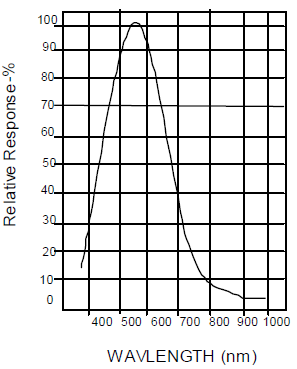
\includegraphics[height=10cm]{figures/komponenter/photosensor}
	\caption{Normal speltral respons angivet i procent}
	Se databladet i kilde \cite{kompPhoto}
	\label{arduinoLCD}
\end{figure}
BPW21 er en fotodiode, som betyder at dens modstand ændres alt efter \todo{skriv teori om BPW21}

\subsubsection{LED - RGB Clear Common Anode}



\subsection{Teori}
\subsubsection{OPAMP}
\subsubsection{Analog input til registrering af farve}
Arduinoens analog input er beskrevet i afsnit \ref{sec:ard:analog}. Vi benytter denne funktion til at få outputtet fra vores farvesensor ind i arduinoen.
\subsection{Beregninger}
\subsubsection{Modstanden af LED}
Ifølge \cite{kompLED} gælder det for LED'en at dens typiske spænding for den blå og grønne LED
\[
	V_{GB typisk} = \SI{3.2}{V}
\]
Og for den røde 
\[
	V_{R typisk} = \SI{2}{V}
\]
Og kan klare en strømstyrke på
\[
	I = \SI{20d-3}{A} 
\]
Ud fra ohms lov må det betyde at hvis indgangsspændingen er på $\SI{5}{V}$, at modstanden til de enkelte LEDer skal være
\begin{align}
	R&= \frac{U}{I}\\
	R_{RLED} &= \frac{\SI{5}{V}-\SI{2}{V}}{\SI{2.0d-2}{A}} = \SI{150}{\ohm}\\
	R_{GLED} &= \frac{\SI{5}{V}-\SI{3.2}{V}}{\SI{2.0d-2}{A}} = \SI{90}{\ohm}\\
	R_{BLED} &= \frac{\SI{5}{V}-\SI{3.2}{V}}{\SI{2.0d-2}{A}} = \SI{90}{\ohm}\\
\end{align}
Ud fra dette valgte vi at benytte modstandene 
\begin{align}
	R_{RLED} &= \SI{180}{\ohm}\\
	R_{GLED} &= \SI{100}{\ohm}\\
	R_{BLED} &= \SI{100}{\ohm}\\
\end{align}
Det vidste sig dog at en LED ikke lyste nok op, og derfor satte vi en ekstra parallelt med den anden som vist på kredsløbstegningen. Dette betød at vi skulle ændre vores modstande, hvor vi også valgte at ændre modstandene således at de 3 forskellige farver tilnærmelsesvis lyste lige stærkt. De nye modstande blev 
\begin{align}
	R_{RLED} &= \SI{120}{\ohm}\\
	R_{GLED} &= \SI{470}{\ohm}\\
	R_{BLED} &= \SI{470}{\ohm}\\
\end{align}
Her blev der lavet en test, af indgangsspændingen til Arduinoen, når der blev lyst med forskellige farver, på materialer med forskellig farve. Testen kan findes i tabel \ref{tab:farveudenforstaerker}.

\subsubsection{OPAMP modstande} \label{subs:opampanalog}
Vi besluttede os for at benytte en OPAMP, da vores største signal fra test 1 (se \ref{tab:farveudenforstaerker}) var på $\SI{0.06}{V}$, hvis man ser bort fra når alle lyser. Da vores precision af analog inputtet på arduinoen er omkring $\SI{0.005}{V}$ (se \ref{sec:ard:analog}), er der små udsving i inputtet, som vi gerne vil gøre større med en OPAMP, så det er nemmere at identificere hvilken farve bliver brugt.
% R_in = 1k
% R_f = 56k
Vi valgte at den maksimale indgangsspænding til OPAMPen er
\[
	V_{in} = \SI{0.08}{V}
\]
Vi ønsker at dette skal være det maksimale som Arduinoen kan måle ($\SI{5}{V}$)
\[
	V_{out} \approx \SI{5}{V}
\]
Heraf er den ønskede forstærkning
\[
	A_{target} = \frac{V_{out}}{V_{in}} = \frac{\SI{5}{V}}{\SI{0.08}{V}}=62.5
\]

Denne forstærkning er ret høj og vi benytter derfor en non-inverting amplifier.

Vi bestemmer en rimelig værdi til den ene modstand er
\begin{align}
	R_{in} = \SI{1000}{\ohm} \label{eq:RinFarveOpAmp}
\end{align}
Og udtrykket for forstærkningen er

\begin{align}
	A_{target} = 1+\frac{R_f}{R_{in}} \label{eq:AtargetFarveOpAmp}
\end{align}
Ved at isolerer $R_f$ i ligningerne \ref{eq:RinFarveOpAmp} og \ref{eq:AtargetFarveOpAmp} fås
\[
	R_f = \SI{61.5d3}{\ohm}
\]
Da vi ikke har denne modstand direkte, vælger vi at benytte en $\SI{56d3}{\ohm}$ modstand i stedet. Hvilket giver os en reel forstærkning på
\[
	A_{reel} = 1 + \frac{\SI{56d3}{\ohm}}{\SI{1000}{\ohm}} = 57	
\]
Hvilket svarer til et outputsignal på
\[
	V_{out} = \SI{0.08}\cdot 57 = \SI{4.56}{V}
\]
Hvilket er tilnærmelsesvis hvad vi gerne vil have. Derefter kørte vi den samme test som før vi havde forstærket signalet. Resultaterne kan ses i tabel \ref{tab:farvemedforstaerker}.





**** NOTER ****
Men da vi satte tre modstande ændrede vi det til ***. 
% MISC LED
Skriv LED anode eller cathode og indsæt tegning 
Simon → Farvesensor
Skriv om bestemmelse af modstande til LED
Start ->
G=100
B=100
R=180

Ændring ->
R=120
G=470
B=470

Skriv om arduino precision (10 bit)-> grunden til brug af opamps

Skriv om opAMP


Nævn af billederne i bilag (grøn blå) blev taget før at afstanden blev ændret fra 6 cm til 3cm.
(afstand 2 cm, mørklagt kasse)
% \usepackage[normalem]{ulem}
% \useunder{\uline}{\ul}{}

*************
\subsection{Test}


\begin{table}[H]
\centering
\caption{Signaler uden forstærkning} \label{tab:farveudenforstaerker}
\label{my-label}
\begin{tabular}{l|lllll}
\hline \hline
     & Alle{[\si{V}]} & Intet {[\si{V}]} & Rød{[\si{V}]} & Grøn{[\si{V}]} & Blå{[\si{V}]} \\
     \hline
Sort & 0.03        & 0.01          & 0.01       & 0.02        & 0.02       \\
Hvid & 0.12        & 0.01          & 0.02       & 0.06        & 0.06       \\
Rød  & 0.03        & 0.01          & 0.02       & 0.01        & 0.02       \\
Blå  & 0.05        & 0.01          & 0.01       & 0.02        & 0.03       \\
Gul  & 0.06        & 0.01          & 0.02       & 0.04        & 0.02       \\
Grøn & 0.04        & 0.01          & 0.01       & 0.03        & 0.02 \\[1ex]
\hline     
\end{tabular}
\end{table}

Test efter forstærkning
% Please add the following required packages to your document preamble:
% \usepackage[normalem]{ulem}
% \useunder{\uline}{\ul}{}
\begin{table}[H]
\centering
\caption{Signaler med forstærkning} \label{tab:farvemedforstaerker}
\begin{tabular}{l|lllll}
\hline\hline
     & Alle{[\si{V}]} & Intet {[\si{V}]} & Rød{[\si{V}]} & Grøn{[\si{V}]} & Blå{[\si{V}]} \\
     \hline
Sort & 0.47        & 0.05          & 0.08       & 0.23        & 0.25       \\
Hvid & 4.8         & 0.04          & 0.77       & 4.04        & 4.38       \\
Rød  & 1.03        & 0.06          & 0.53       & 0.29        & 0.28       \\
Blå  & 2.72        & 0.06          & 0.06       & 0.77        & 1.95       \\
Gul  & 3.8         & 0.06          & 0.75       & 2.42        & 0.75       \\
Grøn & 0.9         & 0.05          & 0.06       & 0.49        & 0.4 \\[1ex]
\hline
\end{tabular}
\end{table}

